\begin{center}
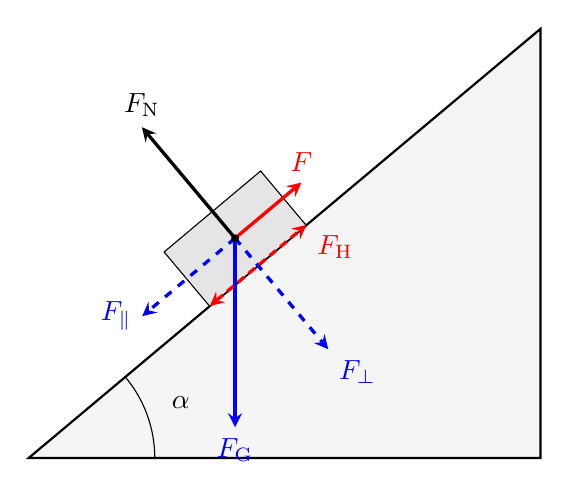
\begin{tikzpicture}[>=stealth]
 \draw[thick, fill=gray!8] (0,0) -- (6.50,0) -- (6.50,5.45) -- cycle;
 \draw (1.6,0) arc (0:40:1.6);
 \node at (1.93,0.70) {$\alpha$};
 \begin{scope}[shift={(2.91,2.44)}, rotate=40]
  \draw[fill=gray!20] (-0.8,0) rectangle (0.8,0.9);
 \end{scope}
 \draw[->, very thick, blue] (2.62,2.79) -- ++(-90.00:2.40) node[anchor=north] {$F_\mathrm{G}$};
 \draw[->, very thick, blue, dashed] (2.62,2.79) -- ++(-50.00:1.84) node[anchor=north west] {$F_\perp$};
 \draw[->, very thick, blue, dashed] (2.62,2.79) -- ++(220.00:1.54) node[anchor=east] {$F_\parallel$};
 \draw[->, very thick, black] (2.62,2.79) -- ++(130.00:1.84) node[anchor=south] {$F_\mathrm{N}$};
 \draw[->, very thick, red] (2.62,2.79) -- ++(40.00:1.10) node[anchor=south] {$F$};
 \fill (2.62,2.79) circle (0.05);
 \draw[<->, very thick, red, densely dashed] (2.30,1.93) -- ++(40:1.6) node[anchor=north west] {$F_\mathrm{H}$};
\end{tikzpicture}
\end{center}

Wir nehmen an, dass die Haltekraft $F$ parallel zur Rampe hangaufwärts wirkt. Die Haftreibungskraft $F_\mathrm{H}$ kann je nach Grösse von $F$ hangaufwärts oder hangabwärts zeigen und höchstens $\mu_\mathrm{H}\,m\,g\cos\alpha$ betragen. Für Holz auf Holz ist $\mu_\mathrm{H} = \muHO$ (FoTaBe S.~189).

\begin{itemize}
\item Kleinste Kraft: Die Kiste droht hinunterzurutschen, die Haftreibung hilft hangaufwärts mit:
 $F_\mathrm{min} + \mu_\mathrm{H}\,m\,g\cos\alpha = m\,g\sin\alpha$.
\item Grösste Kraft: Die Kiste droht hinaufzurutschen, die Haftreibung wirkt hangabwärts:
 $F_\mathrm{max} = m\,g\sin\alpha + \mu_\mathrm{H}\,m\,g\cos\alpha$.
\end{itemize}

Für $\alpha = \wiAO$:
\begin{align}
 F_\mathrm{min} &= \FuAF \\
   &= \mKi\cdot\gE\cdot\left(\sin\left(\wiAO\right)-\muH\cdot\cos\left(\wiAO\right)\right) = \FuA \approx \result{\FuAP{0}{2}} \\
 F_\mathrm{max} &= \FoAF \\
   &= \mKi\cdot\gE\cdot\left(\sin\left(\wiAO\right)+\muH\cdot\cos\left(\wiAO\right)\right) = \FoA \approx \result{\FoAP{0}{2}}
\end{align}
Die Kraft muss also zwischen $\FuAP{0}{2}$ und $\FoAP{0}{2}$ liegen.

Für $\alpha = \wiBO$ geben dieselben Formeln
\begin{align}
 F_\mathrm{min} &= \FuB \approx \FuBP{0}{2} \\
 F_\mathrm{max} &= \FoB \approx \result{\FoBP{0}{2}}
\end{align}
Die untere Grenze ist negativ: Bei \wiBO\ ist $\tan\alpha < \mu_\mathrm{H}$, die Kiste bleibt also auch ohne Kraft liegen. Die Kraft kann zwischen $\result{0}$ und $\FoBP{0}{2}$ hangaufwärts liegen; man könnte die Kiste sogar mit bis zu $\FuBbP{0}{2}$ hangabwärts drücken, ohne dass sie rutscht.

Da $\mu_\mathrm{H}$ für Holz auf Holz stark streut, sind diese Grenzen nur Richtwerte.
